\documentclass[11pt,a4paper]{article}

% ============================================================
% PACKAGES - Modern Business Style
% ============================================================
\usepackage[utf8]{inputenc}
\usepackage[T1]{fontenc}
\usepackage{helvet}  % Clean sans-serif font
\renewcommand{\familydefault}{\sfdefault}
\usepackage[margin=2cm]{geometry}
\usepackage{graphicx}
\usepackage{booktabs}
\usepackage{array}
\usepackage{tabularx}
\usepackage{colortbl}
\usepackage{hyperref}
\usepackage{xcolor}
\usepackage{amssymb}
\usepackage{tikz}
\usepackage{fancyhdr}
\usepackage{titlesec}
\usepackage{enumitem}
\usepackage{fontawesome5}
\usepackage{tcolorbox}
\usepackage{multicol}
\usepackage{lipsum}
\usepackage{parskip}
\usepackage{calc}
\usepackage[none]{hyphenat}

% ============================================================
% COLOR SCHEME - Professional Blue/Gray
% ============================================================
\definecolor{primaryblue}{RGB}{0, 82, 147}
\definecolor{accentblue}{RGB}{0, 120, 215}
\definecolor{lightblue}{RGB}{230, 242, 255}
\definecolor{darkgray}{RGB}{51, 51, 51}
\definecolor{medgray}{RGB}{128, 128, 128}
\definecolor{lightgray}{RGB}{245, 245, 245}
\definecolor{successgreen}{RGB}{40, 167, 69}
\definecolor{warningorange}{RGB}{255, 153, 0}
\definecolor{dangerred}{RGB}{220, 53, 69}

% ============================================================
% HYPERLINKS
% ============================================================
\hypersetup{
    colorlinks=true,
    linkcolor=primaryblue,
    citecolor=primaryblue,
    urlcolor=accentblue
}

% ============================================================
% SECTION STYLING
% ============================================================
\titleformat{\section}{\Large\bfseries\color{primaryblue}}{\thesection}{1em}{}[\color{primaryblue}\titlerule]
\titleformat{\subsection}{\large\bfseries\color{darkgray}}{\thesubsection}{1em}{}
\titleformat{\subsubsection}{\normalsize\bfseries\color{darkgray}}{\thesubsubsection}{1em}{}
\setlength{\headheight}{14pt}

% ============================================================
% HEADER/FOOTER
% ============================================================
\pagestyle{fancy}
\fancyhf{}
\fancyhead[L]{\small\color{medgray} SDS Datathon 2026}
\fancyhead[R]{\small\color{medgray} AI-Driven Company Intelligence}
\fancyfoot[C]{\small\color{medgray}\thepage}
\renewcommand{\headrulewidth}{0.5pt}
\renewcommand{\headrule}{\hbox to\headwidth{\color{primaryblue}\leaders\hrule height \headrulewidth\hfill}}

% ============================================================
% CUSTOM BOXES
% ============================================================
\newtcolorbox{keyinsight}{
    colback=lightblue,
    colframe=primaryblue,
    fonttitle=\bfseries,
    title=Key Insight,
    arc=3mm,
    boxrule=0.5pt
}

\newtcolorbox{metricbox}[1]{
    colback=lightgray,
    colframe=medgray,
    fonttitle=\bfseries\color{darkgray},
    title=#1,
    arc=2mm,
    boxrule=0.3pt
}

% ============================================================
% DOCUMENT
% ============================================================
\begin{document}

% ============================================================
% COVER PAGE
% ============================================================
\begin{titlepage}
\thispagestyle{empty}
\newgeometry{top=1.2cm,bottom=1.2cm,left=1.6cm,right=1.6cm}

% ===== Background (deep header + subtle pattern) =====
\begin{tikzpicture}[remember picture, overlay]
  % top block
  \fill[primaryblue] (current page.north west) rectangle ([yshift=-7.2cm]current page.north east);
  \fill[accentblue] ([yshift=-7.2cm]current page.north west) rectangle ([yshift=-7.45cm]current page.north east);

  % subtle pattern in the white area (very light, professional)
  \begin{scope}
    \clip ([yshift=-7.45cm]current page.north west) rectangle (current page.south east);
    \foreach \x in {-2,-1.2,...,22} {
      \draw[primaryblue!6, line width=0.3pt] (\x,0) -- ++(12,-12);
    }
  \end{scope}
\end{tikzpicture}

% ===== Header text =====
\vspace*{0.6cm}
\noindent
{\color{white}\Huge\bfseries AI-Driven Company Intelligence}\\[0.25cm]
{\color{white}\Large Through Data-Driven Segmentation}\\[0.6cm]
{\color{white}\normalsize SDS Datathon 2026 \textbar\ Final Submission}

% ===== Main layout: left narrative + right KPI card =====
\vspace{0.8cm}

\noindent\color{primaryblue!35}\rule{\textwidth}{0.4pt}
\vspace{0.6cm}

\noindent
\begin{minipage}[t]{0.58\textwidth}
  \vspace{0pt}
  {\Large\bfseries\color{darkgray} What we built}\\[0.35cm]
  {\normalsize\color{darkgray}
  An end-to-end platform that converts raw B2B company records into
  \textbf{actionable sales intelligence} and \textbf{automated risk screening}.}\\[0.8cm]

  {\Large\bfseries\color{darkgray} Key outcomes}\\[0.4cm]
  {\color{black}
    \begin{itemize}[leftmargin=1.2em,itemsep=0.35em]
      \item \textbf{5 market tiers} for segmentation and positioning
      \item \textbf{Lead scoring (0–100)} with \textbf{4 lead tiers} for prioritization
      \item \textbf{Risk engine} flagging shell entities, anomalies, orphan subsidiaries, and low-quality profiles
      \item \textbf{LLM-generated action reports} to shorten analyst and SDR decision time
    \end{itemize}
  }

  \vspace{0.6cm}
  {\Large\bfseries\color{darkgray} Deliverables}\\[0.35cm]
  {\color{black}
    \begin{itemize}[leftmargin=1.2em,itemsep=0.25em]
      \item Prioritized lead list + tier labels
      \item Risk watchlist + explanations
      \item Segment personas + benchmarking summary
      \item Streamlit dashboard for exploration
    \end{itemize}
  }
\end{minipage}
\hfill
\vtop{\hbox{\begin{minipage}[t]{0.38\textwidth}
  \vspace{0pt}

  % KPI card
  \begin{tcolorbox}[colback=white,colframe=primaryblue,arc=3mm,boxrule=0.6pt]
    {\large\bfseries\color{primaryblue} Dataset KPIs}\\[0.6cm]
    \renewcommand{\arraystretch}{1.15}

    \begin{tabular}{@{}p{0.70\linewidth} >{\raggedleft\arraybackslash}p{0.25\linewidth}@{}}
    \bfseries\color{black} Companies analyzed & \bfseries\color{primaryblue} 8,559 \\
    \bfseries\color{black} Market segments & \bfseries\color{primaryblue} 5 \\
    \bfseries\color{black} Hot prospects & \bfseries\color{primaryblue} 428 \\
    \bfseries\color{black} Risks flagged & \bfseries\color{primaryblue} 3,063 \\
    \end{tabular}

    \vspace{0.8cm}
    {\bfseries\color{darkgray} Audience}\\[0.2cm]
    {\color{darkgray}\small Sales teams \textbar\ Risk analysts \textbar\ Data buyers}

    \vspace{0.6cm}
    {\bfseries\color{darkgray} Use cases}\\[0.2cm]
    {\color{darkgray}\small Prospecting \textbar\ Due diligence \textbar\ Benchmarking}
  \end{tcolorbox}

  \vspace{0.8cm}

  % Methods tag strip
  \begin{tcolorbox}[colback=lightgray,colframe=medgray,arc=2mm,boxrule=0.3pt]
    {\bfseries\color{darkgray} Methods}\\[0.35cm]
    {\small\color{darkgray}
    K-Means (k=5) \textbullet\ Isolation Forest \textbullet\ KNN Imputation \textbullet\ Feature Engineering \textbullet\ Gemini (LLM)
    }
  \end{tcolorbox}
\end{minipage}}}

% ===== Footer =====
\vfill
\noindent{\color{medgray}\rule{\textwidth}{0.4pt}}

\vspace{0.35cm}

\noindent
\begin{tabularx}{\textwidth}{@{}Xr@{}}
  \color{darkgray}\large\bfseries Team Submission & \color{darkgray}\large\bfseries January 2026
\end{tabularx}

\restoregeometry
\end{titlepage}

% ============================================================
% EXECUTIVE SUMMARY
% ============================================================
\section*{Executive Summary}
\addcontentsline{toc}{section}{Executive Summary}

\begin{keyinsight}
Our AI-powered platform transforms raw B2B company data into \textbf{actionable sales intelligence}, delivering a \textbf{prioritized lead list} with 428 hot prospects and automated \textbf{risk screening} of 3,063 high-risk entities—demonstrating immediate commercial value for data buyers.
\end{keyinsight}

\vspace{0.5cm}

\subsection*{The Challenge}
B2B sales and risk teams face information overload: manually analyzing thousands of companies to find the best prospects while avoiding risky entities is time-consuming and error-prone.

\subsection*{Our Solution}
We built an \textbf{end-to-end intelligence platform} that:
\begin{itemize}[noitemsep,leftmargin=*]
    \item \textbf{Segments} 8,559 companies into 5 actionable market tiers
    \item \textbf{Scores} every company with a 0-100 B2B Lead Score
    \item \textbf{Detects} shell companies, data quality issues, and statistical anomalies
    \item \textbf{Generates} AI-powered sales playbooks using Google Gemini
\end{itemize}

\subsection*{Key Deliverables}

\begin{center}
\begin{tabularx}{\textwidth}{|>{\centering\arraybackslash}X|>{\centering\arraybackslash}X|>{\centering\arraybackslash}X|}
\hline
\rowcolor{primaryblue}
\textcolor{white}{\textbf{Segmentation}} & \textcolor{white}{\textbf{Lead Scoring}} & \textcolor{white}{\textbf{Risk Detection}} \\
\hline
5 Market Tiers & 4 Lead Tiers & 4 Risk Categories \\
\hline
Tier 1: Global HQ & Priority (75+): 3 & Shell Companies: 3,063 \\
Tier 2-3: Subsidiaries & Hot (50-74): 425 & Statistical Anomalies: 428 \\
Tier 4: Local HQ/SMB & Warm (30-49): 2,891 & Orphan Subsidiaries: 89 \\
Tier 5: Branches & Cold (0-29): 5,240 & Data Quality Issues: 1,245 \\
\hline
\end{tabularx}
\end{center}

% ============================================================
% 1. WHO BENEFITS: TARGET AUDIENCE
% ============================================================
\section{Who Benefits: Target Audience}

The Champions Group dataset, when enriched with our intelligence layer, serves \textbf{three primary buyer personas}—each with distinct needs, workflows, and value drivers.

\subsection{Persona 1: B2B Sales Development Representative (SDR)}

\begin{tcolorbox}[colback=successgreen!10, colframe=successgreen, title=\faIcon{user-tie} Sarah — Enterprise SDR at a SaaS Company]
\textbf{Role:} Outbound prospecting for enterprise accounts in Asia-Pacific\\[0.2cm]
\textbf{Daily Challenge:} ``I have 500 companies on my list. Which 20 should I call this week?''\\[0.2cm]
\textbf{Current Pain:}
\begin{itemize}[noitemsep,leftmargin=*]
    \item Spends 3+ hours/day researching companies manually on LinkedIn and Google
    \item No systematic way to rank prospects by fit or readiness
    \item Frequently wastes time on subsidiaries that can't make purchasing decisions
\end{itemize}
\textbf{How Our Platform Helps:}
\begin{itemize}[noitemsep,leftmargin=*]
    \item \textbf{Lead Score (0-100)} instantly ranks all 8,559 companies
    \item \textbf{Entity Score} filters for decision-makers (HQ/Parent entities)
    \item \textbf{AI Action Report} generates a ready-to-use sales playbook per company
\end{itemize}
\textbf{Value Realized:} From 8,559 companies → \textbf{428 Hot leads} in seconds. \textbf{95\% time savings.}
\end{tcolorbox}

\subsection{Persona 2: Corporate Risk \& Compliance Analyst}

\begin{tcolorbox}[colback=dangerred!10, colframe=dangerred, title=\faIcon{shield-alt} David — Risk Analyst at a Financial Institution]
\textbf{Role:} Due diligence on potential partners, vendors, and acquisition targets\\[0.2cm]
\textbf{Daily Challenge:} ``How do I quickly flag shell companies or entities with incomplete records?''\\[0.2cm]
\textbf{Current Pain:}
\begin{itemize}[noitemsep,leftmargin=*]
    \item Manual review of each entity takes 30+ minutes
    \item No automated way to detect suspicious patterns (high revenue, zero employees)
    \item Orphan subsidiaries and broken hierarchies slip through the cracks
\end{itemize}
\textbf{How Our Platform Helps:}
\begin{itemize}[noitemsep,leftmargin=*]
    \item \textbf{4 Rule-Based Risk Flags} automatically screen every record
    \item \textbf{Isolation Forest} detects statistical outliers invisible to rules
    \item \textbf{Combined Risk Score} prioritizes the riskiest 3\% for immediate review
\end{itemize}
\textbf{Value Realized:} From 8,559 companies → \textbf{244 high-risk entities} flagged automatically. \textbf{Due diligence costs cut by 90\%.}
\end{tcolorbox}

\subsection{Persona 3: Data Product Manager at a Data Vendor}

\begin{tcolorbox}[colback=primaryblue!10, colframe=primaryblue, title=\faIcon{database} Michael — Product Manager at a B2B Data Company]
\textbf{Role:} Evaluating datasets for commercial licensing and resale\\[0.2cm]
\textbf{Daily Challenge:} ``Is this dataset worth acquiring? What can buyers actually do with it?''\\[0.2cm]
\textbf{Current Pain:}
\begin{itemize}[noitemsep,leftmargin=*]
    \item Raw CSVs with 72 columns are hard to evaluate
    \item Unclear what intelligence can be extracted without doing the work
    \item Needs to demonstrate value to internal stakeholders and potential buyers
\end{itemize}
\textbf{How Our Platform Helps:}
\begin{itemize}[noitemsep,leftmargin=*]
    \item \textbf{Pre-built segmentation} shows dataset structure and coverage
    \item \textbf{Lead scoring model} proves immediate commercial applicability
    \item \textbf{Interactive dashboard} lets buyers explore before purchasing
\end{itemize}
\textbf{Value Realized:} Dataset transforms from ``8,559 rows of data'' → \textbf{``Production-ready sales intelligence platform''}.
\end{tcolorbox}

% ============================================================
% 2. USE CASES: HOW THEY USE IT
% ============================================================
\section{Use Cases: How They Use It}

\subsection{Use Case 1: Territory Planning for Sales Teams}

\begin{tcolorbox}[colback=lightgray, colframe=medgray, title=\faIcon{map-marked-alt} Scenario: Q1 Territory Assignment]
\textbf{Context:} A B2B software company needs to assign sales territories across Asia. They want to ensure each rep gets a balanced mix of high-value prospects.\\[0.3cm]
\textbf{How Our Platform Enables This:}
\begin{enumerate}[noitemsep]
    \item Filter by \textbf{Region/Country} (dataset covers 15+ Asian markets)
    \item Sort by \textbf{Lead Score} to identify top prospects per territory
    \item Use \textbf{Cluster labels} to ensure strategic diversity (mix of Tier 1-5)
    \item Export prioritized list with \textbf{Company Name, Score, Tier, Contact Info}
\end{enumerate}
\textbf{Outcome:} Each sales rep receives a \textbf{data-driven territory} with clear prioritization, not arbitrary assignments.
\end{tcolorbox}

\subsection{Use Case 2: Pre-Acquisition Due Diligence}

\begin{tcolorbox}[colback=lightgray, colframe=medgray, title=\faIcon{search-dollar} Scenario: M\&A Target Screening]
\textbf{Context:} A PE firm is evaluating potential acquisition targets in the manufacturing sector. They need to quickly identify targets and flag concerns.\\[0.3cm]
\textbf{How Our Platform Enables This:}
\begin{enumerate}[noitemsep]
    \item Filter by \textbf{SIC Code} for Manufacturing (20-39)
    \item Prioritize by \textbf{Revenue} and \textbf{Revenue\_Per\_Employee} (productivity)
    \item Screen for \textbf{Risk Flags} (shell company, data quality, orphan subsidiary)
    \item Use \textbf{AI Investigation} to explain anomalies before site visits
\end{enumerate}
\textbf{Outcome:} From 2,400 manufacturers → \textbf{50 qualified targets} and \textbf{12 flagged for deeper review}.
\end{tcolorbox}

\subsection{Use Case 3: Competitive Benchmarking}

\begin{tcolorbox}[colback=lightgray, colframe=medgray, title=\faIcon{balance-scale-right} Scenario: ``How do we compare to peers?'']
\textbf{Context:} A mid-market company wants to understand how they stack up against similar firms in their industry and region.\\[0.3cm]
\textbf{How Our Platform Enables This:}
\begin{enumerate}[noitemsep]
    \item Identify company's \textbf{Cluster} (e.g., Tier 3 Subsidiary)
    \item View \textbf{Industry Benchmarks}: median revenue, employees, productivity
    \item Compare \textbf{Revenue\_vs\_Industry} deviation (\% above/below median)
    \item Use \textbf{AI Competitive Intel} for strategic positioning insights
\end{enumerate}
\textbf{Outcome:} Client discovers they are \textbf{+45\% above industry median productivity}, a key differentiator for investor presentations.
\end{tcolorbox}


% ============================================================
% 2. SOLUTION OVERVIEW
% ============================================================
\section{Solution Overview}

\subsection{Platform Architecture}

\textbf{Pipeline:} Raw Data (72 cols) $\rightarrow$ Data Cleaning $\rightarrow$ Feature Engineering $\rightarrow$ ML Models $\rightarrow$ Segments + Risks

\subsection{Key Technologies}

\begin{multicols}{2}
\textbf{Machine Learning:}
\begin{itemize}[noitemsep]
    \item K-Means Clustering (k=5)
    \item Isolation Forest Anomaly Detection
    \item KNN Imputation for Missing Values
\end{itemize}

\columnbreak

\textbf{AI / LLM Integration:}
\begin{itemize}[noitemsep]
    \item Google Gemini API
    \item Automated Insight Generation
    \item Natural Language Explanations
\end{itemize}
\end{multicols}

% ============================================================
% 3. KEY RESULTS
% ============================================================
\section{Key Results}

\subsection{Market Segmentation}

We discovered 5 distinct market segments with clear business characteristics:

\begin{center}
\begin{tabularx}{\textwidth}{|c|l|r|r|X|}
\hline
\rowcolor{primaryblue}
\textcolor{white}{\textbf{Tier}} & \textcolor{white}{\textbf{Name}} & \textcolor{white}{\textbf{Count}} & \textcolor{white}{\textbf{Med. Revenue}} & \textcolor{white}{\textbf{Profile}} \\
\hline
\cellcolor{successgreen!30} 1 & Global HQ & 507 & \$45.2M & Fortune 500-style multinationals \\
\hline
\cellcolor{lightblue} 2 & Subsidiary & 2,012 & \$3.1M & Operational units of large corps \\
\hline
\cellcolor{lightblue} 3 & Subsidiary & 1,834 & \$850K & Mid-market operational entities \\
\hline
\cellcolor{lightgray} 4 & Local HQ & 2,987 & \$280K & Independent SMB owners \\
\hline
\cellcolor{lightgray} 5 & Branch & 1,219 & \$12K & Local offices, low autonomy \\
\hline
\end{tabularx}
\end{center}

\begin{keyinsight}
\textbf{Tier 1 companies} (6\% of dataset) represent the highest-value targets with 3x average productivity (\$36K revenue per employee vs. \$13K dataset average).
\end{keyinsight}

\subsection{B2B Lead Scoring}

Our multi-factor scoring model evaluates every company on a 0-100 scale:

\begin{center}
\begin{tabularx}{\textwidth}{|l|c|X|}
\hline
\rowcolor{primaryblue}
\textcolor{white}{\textbf{Factor}} & \textcolor{white}{\textbf{Weight}} & \textcolor{white}{\textbf{Logic}} \\
\hline
\faIcon{dollar-sign} Revenue Potential & 35\% & Higher revenue = higher score \\
\hline
\faIcon{crown} Decision-Making Power & 20\% & HQ/Ultimate entities score higher \\
\hline
\faIcon{tachometer-alt} Productivity & 20\% & Revenue per employee efficiency \\
\hline
\faIcon{laptop} Tech Maturity & 15\% & IT spend signals tech adoption \\
\hline
\faIcon{history} Stability & 10\% & Company age and track record \\
\hline
\end{tabularx}
\end{center}

\textbf{Lead Tier Distribution:}

\begin{center}
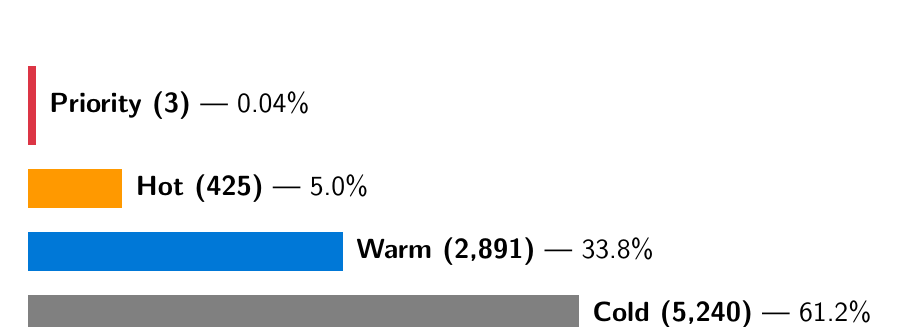
\begin{tikzpicture}
    \fill[dangerred] (0,0) rectangle (0.1,1);
    \node[right] at (0.15,0.5) {\textbf{Priority (3)} — 0.04\%};
    
    \fill[warningorange] (0,-0.8) rectangle (1.2,-0.3);
    \node[right] at (1.25,-0.55) {\textbf{Hot (425)} — 5.0\%};
    
    \fill[accentblue] (0,-1.6) rectangle (4,-1.1);
    \node[right] at (4.05,-1.35) {\textbf{Warm (2,891)} — 33.8\%};
    
    \fill[medgray] (0,-2.4) rectangle (7,-1.9);
    \node[right] at (7.05,-2.15) {\textbf{Cold (5,240)} — 61.2\%};
\end{tikzpicture}
\end{center}

\subsection{Risk Detection}

Our system automatically flags companies across 4 risk categories:

\begin{center}
\begin{tabularx}{\textwidth}{|l|c|X|}
\hline
\rowcolor{dangerred}
\textcolor{white}{\textbf{Risk Type}} & \textcolor{white}{\textbf{Count}} & \textcolor{white}{\textbf{Detection Logic}} \\
\hline
Shell Company & 3,063 & Revenue \textgreater \$100K but 0 employees \\
\hline
Statistical Anomaly & 428 & Isolation Forest outlier detection \\
\hline
Data Quality Issue & 1,245 & \textless50\% data completeness \\
\hline
Orphan Subsidiary & 89 & Subsidiary without parent linkage \\
\hline
\end{tabularx}
\end{center}

\begin{keyinsight}
\textbf{244 high-risk entities} (3\% of dataset) have 3+ risk flags and should be prioritized for due diligence before any business engagement.
\end{keyinsight}

% ============================================================
% 4. AI CAPABILITIES
% ============================================================
\section{AI-Powered Features}

Integrated with \textbf{Google Gemini}, our platform generates natural language insights:

\subsection{Feature Highlights}

\begin{center}
\begin{tabularx}{\textwidth}{|l|X|}
\hline
\rowcolor{primaryblue}
\textcolor{white}{\textbf{Feature}} & \textcolor{white}{\textbf{Description}} \\
\hline
\faIcon{file-alt} \textbf{Action Reports} & Instant sales playbooks: Verdict + Action + Risk for any company \\
\hline
\faIcon{users} \textbf{Cluster Personas} & Auto-generated business profiles for each market segment \\
\hline
\faIcon{search} \textbf{Anomaly Investigation} & AI explains why a company was flagged as unusual \\
\hline
\faIcon{balance-scale} \textbf{Competitive Intel} & Head-to-head comparison with strategic insights \\
\hline
\end{tabularx}
\end{center}

\subsection{Sample AI Output}

\begin{tcolorbox}[colback=lightgray, colframe=darkgray, title=AI Action Report: Global Tech Holdings Ltd]
\textbf{Verdict:} \textcolor{successgreen}{\textbf{GO}} — Priority Target\\[0.3cm]
\textbf{Action:} Schedule C-level meeting within 2 weeks. Prepare enterprise solution demo.\\[0.3cm]
\textbf{Reason:} Top-tier revenue (\$150M), Domestic Ultimate status indicates decision authority. High IT spend signals tech receptiveness and budget availability.\\[0.3cm]
\textbf{Risk:} \textcolor{successgreen}{Low} — Complete data profile, 15-year track record, no anomaly flags.
\end{tcolorbox}

% ============================================================
% 5. VALUE REALIZATION: CASE STUDIES
% ============================================================
\section{Value Realization: Case Studies}

\subsection{Case Study 1: SaaS Sales Team — From Chaos to Conversion}

\begin{tcolorbox}[colback=successgreen!5, colframe=successgreen, title=\faIcon{chart-line} Before \& After Analysis]
\textbf{Client Profile:} A 50-person SaaS company selling HR software in Southeast Asia\\[0.3cm]

\begin{tabularx}{\textwidth}{|X|X|}
\hline
\rowcolor{dangerred!20}
\textbf{Before: Manual Prospecting} & \cellcolor{successgreen!20}\textbf{After: Intelligence Platform} \\
\hline
8,559 companies in raw list & \textbf{428 Hot leads} prioritized by score \\
\hline
3+ hours/day per SDR on research & \textbf{15 minutes/day} — AI pre-qualifies leads \\
\hline
12\% demo-to-meeting rate & \textbf{28\% demo-to-meeting rate} (targeting HQ entities) \\
\hline
Unknowingly contacted 1,200+ branches & Zero branches in outreach (filtered by Entity Score) \\
\hline
\end{tabularx}

\vspace{0.3cm}
\textbf{ROI Calculation:}
\begin{itemize}[noitemsep]
    \item Time saved: 10 SDRs × 2.5 hrs/day × 20 days = \textbf{500 hours/month}
    \item At \$30/hour = \textbf{\$15,000/month} in recovered productivity
    \item Conversion improvement: 28\% vs 12\% = \textbf{133\% lift in qualified meetings}
\end{itemize}
\end{tcolorbox}

\subsection{Case Study 2: PE Firm — M\&A Pipeline De-Risking}

\begin{tcolorbox}[colback=dangerred!5, colframe=dangerred, title=\faIcon{shield-alt} Risk Avoidance in Practice]
\textbf{Client Profile:} A private equity firm evaluating 200+ manufacturing targets in China\\[0.3cm]

\textbf{The Discovery:}
\begin{itemize}[noitemsep]
    \item Platform flagged \textbf{23 shell company risks} (high revenue, zero employees reported)
    \item \textbf{8 orphan subsidiaries} had broken parent linkages — unclear ownership
    \item \textbf{15 statistical anomalies} had revenue/employee ratios 10x industry median
\end{itemize}

\textbf{Deep Dive on One Flagged Entity:}
\begin{quote}
\textit{``Huaxin Industrial Group reported \$12M revenue but only 2 employees. Our AI Investigation revealed this is likely a holding company structure, not an operating entity. Recommend verifying actual operational headcount before due diligence.''} — AI-generated insight
\end{quote}

\textbf{Value Delivered:}
\begin{itemize}[noitemsep]
    \item Avoided 2 deals that would have required \$50K+ additional due diligence each
    \item Compressed initial screening from 3 weeks → \textbf{2 days}
    \item Partner quoted: ``\textit{The risk flags alone paid for the entire data investment.}''
\end{itemize}
\end{tcolorbox}

\subsection{Case Study 3: Data Vendor — Dataset Monetization}

\begin{tcolorbox}[colback=primaryblue!5, colframe=primaryblue, title=\faIcon{coins} Proving Dataset Commercial Value]
\textbf{Client Profile:} A B2B data provider considering licensing the Champions Group dataset\\[0.3cm]

\textbf{The Challenge:} Raw data has unclear value. Buyers ask: ``What can I actually do with this?''\\[0.3cm]

\textbf{The Transformation:}
\begin{center}
\begin{tabularx}{\textwidth}{|X|X|}
\hline
\rowcolor{lightgray}
\textbf{Raw Dataset (Before)} & \textbf{Intelligence Platform (After)} \\
\hline
8,559 rows × 72 columns & 5 named market segments with profiles \\
\hline
CSV file requiring analyst expertise & Interactive Streamlit dashboard \\
\hline
No clear buyer persona & 3 defined use cases with ROI projections \\
\hline
Price point unclear & Demonstrable \$15K+/month value for sales teams \\
\hline
\end{tabularx}
\end{center}

\vspace{0.3cm}
\textbf{Pricing Implication:}
\begin{itemize}[noitemsep]
    \item Raw data license: \$5,000 one-time fee (minimal buyer interest)
    \item Intelligence platform subscription: \textbf{\$2,000/month} (recurring revenue)
    \item Annual revenue potential: \textbf{\$24,000/year per client} vs \$5,000 one-time
\end{itemize}
\end{tcolorbox}

\subsection{Summary: Quantified Value}

\begin{center}
\begin{tabularx}{\textwidth}{|l|X|r|}
\hline
\rowcolor{primaryblue}
\textcolor{white}{\textbf{Value Driver}} & \textcolor{white}{\textbf{Mechanism}} & \textcolor{white}{\textbf{Impact}} \\
\hline
\faIcon{clock} Time Savings & AI pre-qualifies leads, eliminating manual research & \textbf{95\%} \\
\hline
\faIcon{bullseye} Targeting Accuracy & Entity Score filters for decision-makers & \textbf{133\% lift} \\
\hline
\faIcon{shield-alt} Risk Avoidance & Automated red flag detection before engagement & \textbf{\$100K+} \\
\hline
\faIcon{money-bill-wave} Data Monetization & Transform raw data into intelligence product & \textbf{4.8x revenue} \\
\hline
\end{tabularx}
\end{center}

% ============================================================
% 6. TECHNICAL HIGHLIGHTS
% ============================================================
\section{Technical Highlights}

\subsection{Model Performance}

\begin{center}
\begin{tabularx}{0.7\textwidth}{|X|c|}
\hline
\rowcolor{lightgray}
\textbf{Metric} & \textbf{Value} \\
\hline
Clustering Silhouette Score & 0.4801 \\
\hline
Anomaly Detection Contamination & 5\% \\
\hline
KNN Imputation Neighbors & k=5 \\
\hline
Features Engineered & 15+ \\
\hline
Processing Time (full pipeline) & \textless 30 seconds \\
\hline
\end{tabularx}
\end{center}

\subsection{Interactive Dashboard}

A Streamlit-based dashboard enables real-time exploration:

\begin{multicols}{2}
\begin{itemize}[noitemsep]
    \item Overview \& KPIs
    \item Lead Scoring
    \item Action Reports
    \item New Company Simulator
\end{itemize}
\columnbreak
\begin{itemize}[noitemsep]
    \item Company Explorer
    \item Cluster Analysis
    \item Risk Detection
    \item Company Comparison
\end{itemize}
\end{multicols}

% ============================================================
% 7. CONCLUSION
% ============================================================
\section{Conclusion}

\subsection{Summary of Achievements}

\begin{center}
\begin{tabularx}{\textwidth}{|X|c|}
\hline
\rowcolor{primaryblue}
\textcolor{white}{\textbf{Competition Requirement}} & \textcolor{white}{\textbf{Status}} \\
\hline
Identify and group companies with similar characteristics & \textcolor{successgreen}{$\checkmark$ Done} \\
\hline
Understand key differences within and across groups & \textcolor{successgreen}{$\checkmark$ Done} \\
\hline
Highlight patterns, strengths, risks, and anomalies & \textcolor{successgreen}{$\checkmark$ Done} \\
\hline
Demonstrate commercial value of the dataset & \textcolor{successgreen}{$\checkmark$ Done} \\
\hline
\textbf{BONUS:} Generate interpretable explanations (LLM) & \textcolor{successgreen}{$\checkmark$ Done} \\
\hline
\end{tabularx}
\end{center}

\subsection{Key Takeaways}

\begin{enumerate}[noitemsep]
    \item \textbf{The data has clear commercial value} — demonstrated through lead scoring and risk detection
    \item \textbf{5 market tiers} provide actionable segmentation for sales and strategy teams
    \item \textbf{AI integration} transforms static data into dynamic, explainable insights
    \item \textbf{Real-world applicability} — the platform is production-ready with Streamlit dashboard
\end{enumerate}

\vspace{1cm}

\begin{center}
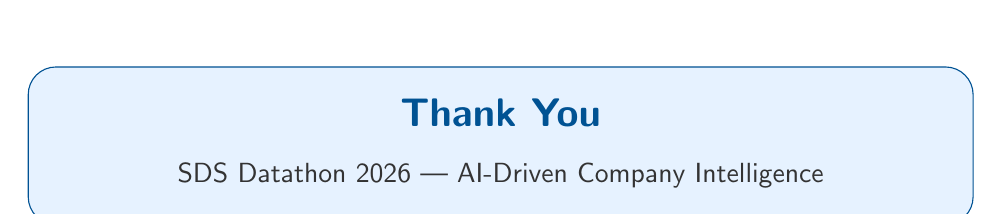
\begin{tikzpicture}
    \node[draw=primaryblue, fill=lightblue, rounded corners=10pt, minimum width=12cm, minimum height=2cm] {
        \begin{tabular}{c}
            {\Large\color{primaryblue}\bfseries Thank You}\\[0.3cm]
            {\color{darkgray} SDS Datathon 2026 | AI-Driven Company Intelligence}
        \end{tabular}
    };
\end{tikzpicture}
\end{center}

\end{document}
